\documentclass[a4paper]{article}

%================================================================================================================================
%
% Packages
%
%================================================================================================================================

\usepackage[T1]{fontenc} 	% pour caractères accentués
\usepackage[utf8]{inputenc}  % encodage utf8
\usepackage[french]{babel}	% langue : français
\usepackage{fourier}			% caractères plus lisibles
\usepackage[dvipsnames]{xcolor} % couleurs
\usepackage{fancyhdr}		% réglage header footer
\usepackage{needspace}		% empêcher sauts de page mal placés
\usepackage{graphicx}		% pour inclure des graphiques
\usepackage{enumitem,cprotect}		% personnalise les listes d'items (nécessaire pour ol, al ...)
\usepackage{hyperref}		% Liens hypertexte
\usepackage{pstricks,pst-all,pst-node,pstricks-add,pst-math,pst-plot,pst-tree,pst-eucl} % pstricks
\usepackage[a4paper,includeheadfoot,top=2cm,left=3cm, bottom=2cm,right=3cm]{geometry} % marges etc.
\usepackage{comment}			% commentaires multilignes
\usepackage{amsmath,environ} % maths (matrices, etc.)
\usepackage{amssymb,makeidx}
\usepackage{bm}				% bold maths
\usepackage{tabularx}		% tableaux
\usepackage{colortbl}		% tableaux en couleur
\usepackage{fontawesome}		% Fontawesome
\usepackage{environ}			% environment with command
\usepackage{fp}				% calculs pour ps-tricks
\usepackage{multido}			% pour ps tricks
\usepackage[np]{numprint}	% formattage nombre
\usepackage{tikz,tkz-tab} 			% package principal TikZ
\usepackage{pgfplots}   % axes
\usepackage{mathrsfs}    % cursives
\usepackage{calc}			% calcul taille boites
\usepackage[scaled=0.875]{helvet} % font sans serif
\usepackage{svg} % svg
\usepackage{scrextend} % local margin
\usepackage{scratch} %scratch
\usepackage{multicol} % colonnes
%\usepackage{infix-RPN,pst-func} % formule en notation polanaise inversée
\usepackage{listings}

%================================================================================================================================
%
% Réglages de base
%
%================================================================================================================================

\lstset{
language=Python,   % R code
literate=
{á}{{\'a}}1
{à}{{\`a}}1
{ã}{{\~a}}1
{é}{{\'e}}1
{è}{{\`e}}1
{ê}{{\^e}}1
{í}{{\'i}}1
{ó}{{\'o}}1
{õ}{{\~o}}1
{ú}{{\'u}}1
{ü}{{\"u}}1
{ç}{{\c{c}}}1
{~}{{ }}1
}


\definecolor{codegreen}{rgb}{0,0.6,0}
\definecolor{codegray}{rgb}{0.5,0.5,0.5}
\definecolor{codepurple}{rgb}{0.58,0,0.82}
\definecolor{backcolour}{rgb}{0.95,0.95,0.92}

\lstdefinestyle{mystyle}{
    backgroundcolor=\color{backcolour},   
    commentstyle=\color{codegreen},
    keywordstyle=\color{magenta},
    numberstyle=\tiny\color{codegray},
    stringstyle=\color{codepurple},
    basicstyle=\ttfamily\footnotesize,
    breakatwhitespace=false,         
    breaklines=true,                 
    captionpos=b,                    
    keepspaces=true,                 
    numbers=left,                    
xleftmargin=2em,
framexleftmargin=2em,            
    showspaces=false,                
    showstringspaces=false,
    showtabs=false,                  
    tabsize=2,
    upquote=true
}

\lstset{style=mystyle}


\lstset{style=mystyle}
\newcommand{\imgdir}{C:/laragon/www/newmc/assets/imgsvg/}
\newcommand{\imgsvgdir}{C:/laragon/www/newmc/assets/imgsvg/}

\definecolor{mcgris}{RGB}{220, 220, 220}% ancien~; pour compatibilité
\definecolor{mcbleu}{RGB}{52, 152, 219}
\definecolor{mcvert}{RGB}{125, 194, 70}
\definecolor{mcmauve}{RGB}{154, 0, 215}
\definecolor{mcorange}{RGB}{255, 96, 0}
\definecolor{mcturquoise}{RGB}{0, 153, 153}
\definecolor{mcrouge}{RGB}{255, 0, 0}
\definecolor{mclightvert}{RGB}{205, 234, 190}

\definecolor{gris}{RGB}{220, 220, 220}
\definecolor{bleu}{RGB}{52, 152, 219}
\definecolor{vert}{RGB}{125, 194, 70}
\definecolor{mauve}{RGB}{154, 0, 215}
\definecolor{orange}{RGB}{255, 96, 0}
\definecolor{turquoise}{RGB}{0, 153, 153}
\definecolor{rouge}{RGB}{255, 0, 0}
\definecolor{lightvert}{RGB}{205, 234, 190}
\setitemize[0]{label=\color{lightvert}  $\bullet$}

\pagestyle{fancy}
\renewcommand{\headrulewidth}{0.2pt}
\fancyhead[L]{maths-cours.fr}
\fancyhead[R]{\thepage}
\renewcommand{\footrulewidth}{0.2pt}
\fancyfoot[C]{}

\newcolumntype{C}{>{\centering\arraybackslash}X}
\newcolumntype{s}{>{\hsize=.35\hsize\arraybackslash}X}

\setlength{\parindent}{0pt}		 
\setlength{\parskip}{3mm}
\setlength{\headheight}{1cm}

\def\ebook{ebook}
\def\book{book}
\def\web{web}
\def\type{web}

\newcommand{\vect}[1]{\overrightarrow{\,\mathstrut#1\,}}

\def\Oij{$\left(\text{O}~;~\vect{\imath},~\vect{\jmath}\right)$}
\def\Oijk{$\left(\text{O}~;~\vect{\imath},~\vect{\jmath},~\vect{k}\right)$}
\def\Ouv{$\left(\text{O}~;~\vect{u},~\vect{v}\right)$}

\hypersetup{breaklinks=true, colorlinks = true, linkcolor = OliveGreen, urlcolor = OliveGreen, citecolor = OliveGreen, pdfauthor={Didier BONNEL - https://www.maths-cours.fr} } % supprime les bordures autour des liens

\renewcommand{\arg}[0]{\text{arg}}

\everymath{\displaystyle}

%================================================================================================================================
%
% Macros - Commandes
%
%================================================================================================================================

\newcommand\meta[2]{    			% Utilisé pour créer le post HTML.
	\def\titre{titre}
	\def\url{url}
	\def\arg{#1}
	\ifx\titre\arg
		\newcommand\maintitle{#2}
		\fancyhead[L]{#2}
		{\Large\sffamily \MakeUppercase{#2}}
		\vspace{1mm}\textcolor{mcvert}{\hrule}
	\fi 
	\ifx\url\arg
		\fancyfoot[L]{\href{https://www.maths-cours.fr#2}{\black \footnotesize{https://www.maths-cours.fr#2}}}
	\fi 
}


\newcommand\TitreC[1]{    		% Titre centré
     \needspace{3\baselineskip}
     \begin{center}\textbf{#1}\end{center}
}

\newcommand\newpar{    		% paragraphe
     \par
}

\newcommand\nosp {    		% commande vide (pas d'espace)
}
\newcommand{\id}[1]{} %ignore

\newcommand\boite[2]{				% Boite simple sans titre
	\vspace{5mm}
	\setlength{\fboxrule}{0.2mm}
	\setlength{\fboxsep}{5mm}	
	\fcolorbox{#1}{#1!3}{\makebox[\linewidth-2\fboxrule-2\fboxsep]{
  		\begin{minipage}[t]{\linewidth-2\fboxrule-4\fboxsep}\setlength{\parskip}{3mm}
  			 #2
  		\end{minipage}
	}}
	\vspace{5mm}
}

\newcommand\CBox[4]{				% Boites
	\vspace{5mm}
	\setlength{\fboxrule}{0.2mm}
	\setlength{\fboxsep}{5mm}
	
	\fcolorbox{#1}{#1!3}{\makebox[\linewidth-2\fboxrule-2\fboxsep]{
		\begin{minipage}[t]{1cm}\setlength{\parskip}{3mm}
	  		\textcolor{#1}{\LARGE{#2}}    
 	 	\end{minipage}  
  		\begin{minipage}[t]{\linewidth-2\fboxrule-4\fboxsep}\setlength{\parskip}{3mm}
			\raisebox{1.2mm}{\normalsize\sffamily{\textcolor{#1}{#3}}}						
  			 #4
  		\end{minipage}
	}}
	\vspace{5mm}
}

\newcommand\cadre[3]{				% Boites convertible html
	\par
	\vspace{2mm}
	\setlength{\fboxrule}{0.1mm}
	\setlength{\fboxsep}{5mm}
	\fcolorbox{#1}{white}{\makebox[\linewidth-2\fboxrule-2\fboxsep]{
  		\begin{minipage}[t]{\linewidth-2\fboxrule-4\fboxsep}\setlength{\parskip}{3mm}
			\raisebox{-2.5mm}{\sffamily \small{\textcolor{#1}{\MakeUppercase{#2}}}}		
			\par		
  			 #3
 	 		\end{minipage}
	}}
		\vspace{2mm}
	\par
}

\newcommand\bloc[3]{				% Boites convertible html sans bordure
     \needspace{2\baselineskip}
     {\sffamily \small{\textcolor{#1}{\MakeUppercase{#2}}}}    
		\par		
  			 #3
		\par
}

\newcommand\CHelp[1]{
     \CBox{Plum}{\faInfoCircle}{À RETENIR}{#1}
}

\newcommand\CUp[1]{
     \CBox{NavyBlue}{\faThumbsOUp}{EN PRATIQUE}{#1}
}

\newcommand\CInfo[1]{
     \CBox{Sepia}{\faArrowCircleRight}{REMARQUE}{#1}
}

\newcommand\CRedac[1]{
     \CBox{PineGreen}{\faEdit}{BIEN R\'EDIGER}{#1}
}

\newcommand\CError[1]{
     \CBox{Red}{\faExclamationTriangle}{ATTENTION}{#1}
}

\newcommand\TitreExo[2]{
\needspace{4\baselineskip}
 {\sffamily\large EXERCICE #1\ (\emph{#2 points})}
\vspace{5mm}
}

\newcommand\img[2]{
          \includegraphics[width=#2\paperwidth]{\imgdir#1}
}

\newcommand\imgsvg[2]{
       \begin{center}   \includegraphics[width=#2\paperwidth]{\imgsvgdir#1} \end{center}
}


\newcommand\Lien[2]{
     \href{#1}{#2 \tiny \faExternalLink}
}
\newcommand\mcLien[2]{
     \href{https~://www.maths-cours.fr/#1}{#2 \tiny \faExternalLink}
}

\newcommand{\euro}{\eurologo{}}

%================================================================================================================================
%
% Macros - Environement
%
%================================================================================================================================

\newenvironment{tex}{ %
}
{%
}

\newenvironment{indente}{ %
	\setlength\parindent{10mm}
}

{
	\setlength\parindent{0mm}
}

\newenvironment{corrige}{%
     \needspace{3\baselineskip}
     \medskip
     \textbf{\textsc{Corrigé}}
     \medskip
}
{
}

\newenvironment{extern}{%
     \begin{center}
     }
     {
     \end{center}
}

\NewEnviron{code}{%
	\par
     \boite{gray}{\texttt{%
     \BODY
     }}
     \par
}

\newenvironment{vbloc}{% boite sans cadre empeche saut de page
     \begin{minipage}[t]{\linewidth}
     }
     {
     \end{minipage}
}
\NewEnviron{h2}{%
    \needspace{3\baselineskip}
    \vspace{0.6cm}
	\noindent \MakeUppercase{\sffamily \large \BODY}
	\vspace{1mm}\textcolor{mcgris}{\hrule}\vspace{0.4cm}
	\par
}{}

\NewEnviron{h3}{%
    \needspace{3\baselineskip}
	\vspace{5mm}
	\textsc{\BODY}
	\par
}

\NewEnviron{margeneg}{ %
\begin{addmargin}[-1cm]{0cm}
\BODY
\end{addmargin}
}

\NewEnviron{html}{%
}

\begin{document}
\meta{url}{/exercices/fonctions-bac-blanc-es-l-sujet-1-maths-cours-2017/}
\meta{pid}{10394}
\meta{titre}{Fonctions - Bac blanc ES/L Sujet 1 - Maths-cours 2017}
\meta{type}{exercices}
%
\begin{h2}Exercice 2 (5 points)\end{h2}
\par
\medskip
\par
Une entreprise produit et commercialise des granulés de céréales destinés à l'alimentation des volailles.
\par
Elle produit, chaque jour, entre 0 et 5 tonnes de granulés.
\par
On note $x$ le nombre de tonnes de granulés produits quotidiennement par cette entreprise.
\par
Le coût de fabrication quotidien, en centaines d'euros peut être modélisé par une fonction $C$, définie sur l'intervalle $[0~;~5]$  dont la représentation graphique $\mathscr{C}$ est fournie en \textbf{Annexe} (voir à la fin du sujet).
\par
L'entreprise vend la totalité des granulés produits au prix de 5 400 euros la tonne.
\par
%============================================================================================================================
%
\TitreC{Partie A}
%
%============================================================================================================================
\par
\begin{enumerate}
     \item Expliquer pourquoi la recette quotidienne de l'entreprise peut être modélisée par la fonction $R$ définie sur l'intervalle $[0~;~5]$ par~:
     \[ R(x)= 54x \]
     Tracer la représentation $\mathscr{R}$ de la fonction $R$ sur le graphique fourni en annexe 1 (à rendre avec la copie).
     \par
     \medskip
     \par
     \item Estimer, à l'aide du graphique, le coût de fabrication quotidien et la recette quotidienne pour une production de 2 tonnes puis de 5 tonnes.
     \par
     Indiquer, dans chacun de ces deux cas, si l'entreprise est bénéficiaire.
     \par
     \medskip
     \par
     \item Par lecture graphique, estimer l'intervalle auquel doit appartenir $x$ pour que l'entreprise réalise un bénéfice.
\end{enumerate}
\par
%============================================================================================================================
%
\TitreC{Partie B}
%
%============================================================================================================================
\par
Dans cette partie, on suppose que le coût de fabrication de $x$ tonnes de granulés, en centaines d'euros, peut être modélisé sur l'intervalle $[0~;~5]$ par~:
\[ C(x)=8x^3-60x^2+150x \]
\begin{enumerate}
     \item Calculer $C'(x)$.
     \par
     En déduire que la fonction $C$ est croissante sur $[0~;~5]$.
     \par
     \medskip
     \par
     \item On note $B(x)$ le résultat net quotidien (en centaines d'euros) de l'entreprise, c'est à dire la différence entre la recette et le coût de fabrication quotidien.
     \par
     Exprimer $B(x)$ puis $B'(x)$ en fonction de $x$.
     \par
     \medskip
     \par
     \item Tracer le tableau de variations de la fonction $B$ sur l'intervalle $[0~;~5]$.
     \par
     \medskip
     \par
     \item Pour quelle production le résultat net de l'entreprise est-t-il maximal ?
     \par
     Quel est alors ce maximum ?
     \par
     \medskip
     \par
\end{enumerate}
%
%============================================================================================================================
%
%			Annexe
%
%============================================================================================================================
%
\TitreC{ANNEXE}
%
\medskip
%
\begin{center}
     \emph{\`A rendre avec la copie}
\end{center}
%
\bigskip
%
\begin{center}
     \begin{extern}%width="600" alt="Courbe résultats nets-bénéfices"
          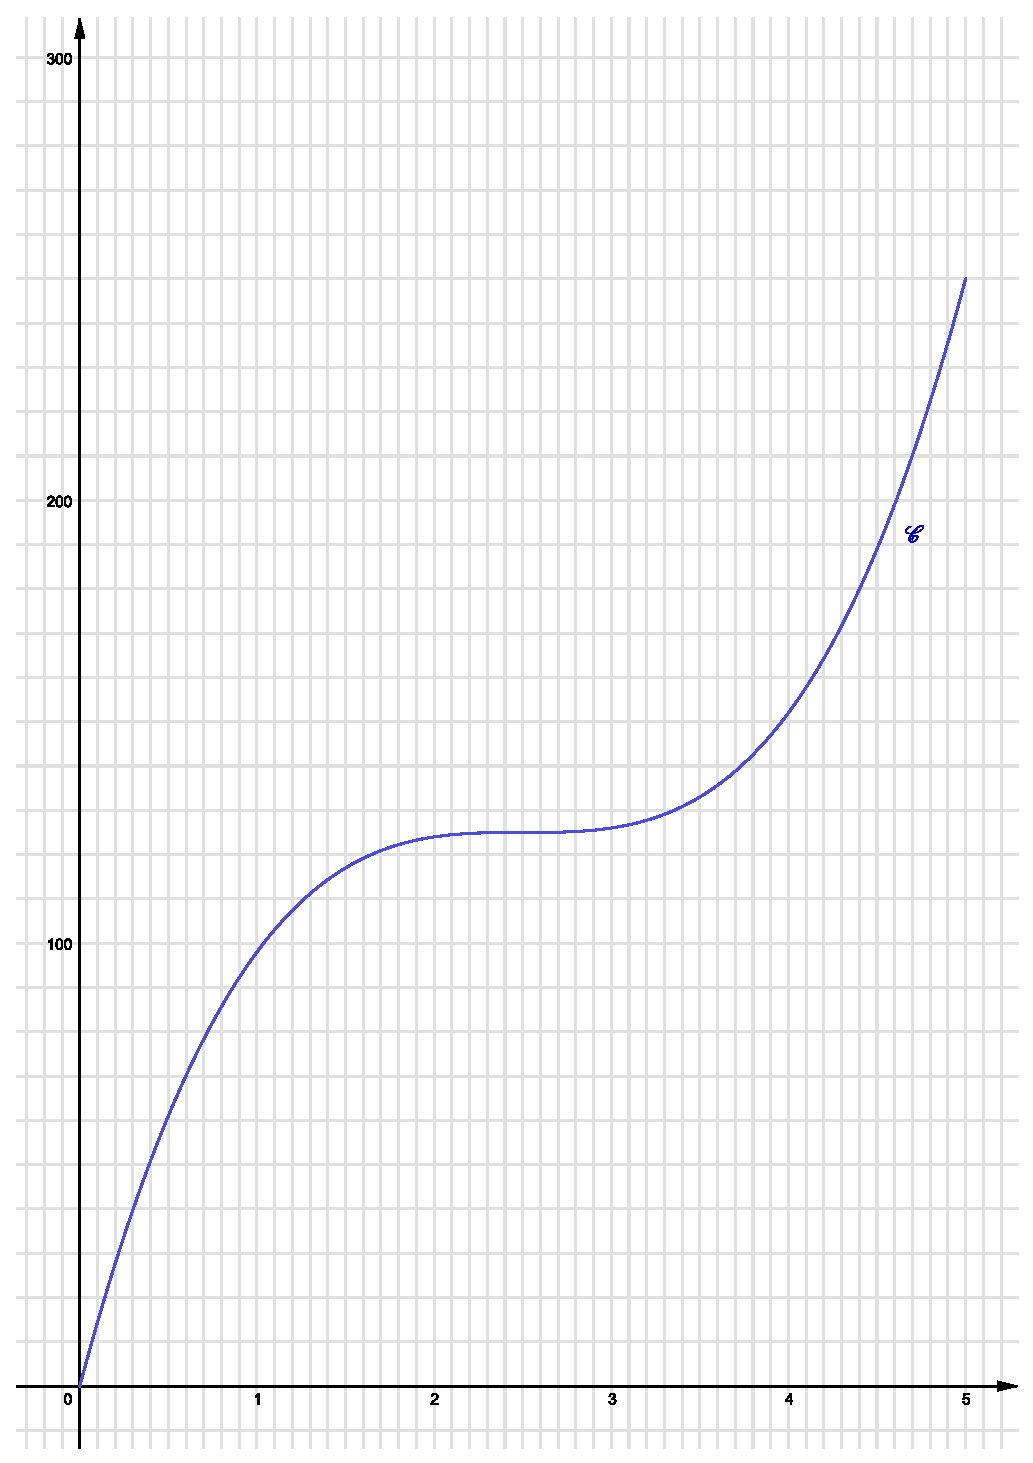
\includegraphics[width=10cm]{images/BBESL-s1-2-1.eps}% gbb 1 unite=3cm
     \end{extern}
\end{center}
\begin{center}
\imgsvg{BBESL-s1-1-1}{0.3}% alt="QCM - Bac blanc ES/L Sujet 1 " style="width:50rem"
\end{center}
%
\begin{corrige}
     %============================================================================================================================
     %
     \TitreC{Partie A}
     %
     %============================================================================================================================
     \par
     \begin{enumerate}
          \item Pour une tonne de granulés, l'entreprise encaisse $5\ 400$~euros soit {$54$ centaines} d'euros.
          \par
          Comme l'entreprise produit et vend quotidiennement $x$ tonnes de granulés (avec $0 \leqslant x \leqslant 5$), la recette quotidienne de l'entreprise, en centaines d'euros, peut être modélisée par la fonction $R$ définie sur l'intervalle $[0~;~5]$ par~:
          \[ R(x)= 54x.\]
          \par
          Cette fonction est la restriction à l'intervalle $[0~;~5]$ d'une \textbf{fonction linéaire}.
          \par
          \cadre{rouge}{Bien rédiger}{
               Lorsque vous rencontrez une fonction étudiée en cours (fonction linéaire, affine, carré, inverse, polynôme du second degré, ...), indiquez-le clairement sur votre copie.
               \par
               Cela vous permettra notamment de justifier l'allure de la courbe représentative (droite, hyperbole, parabole, ...).
          }
          \par
          Sa représentation graphique $\mathscr{R}$ est un segment de \textbf{droite passant par l'origine}.
          \par
          Pour $x=5$, la recette est $R(5)=270$ ; donc la droite passe par le point de coordonnées $(5~;~270)$ (voir graphique).
          \begin{center}
               \begin{extern}%width="600" alt="Lecture graphique coût-recette"
                    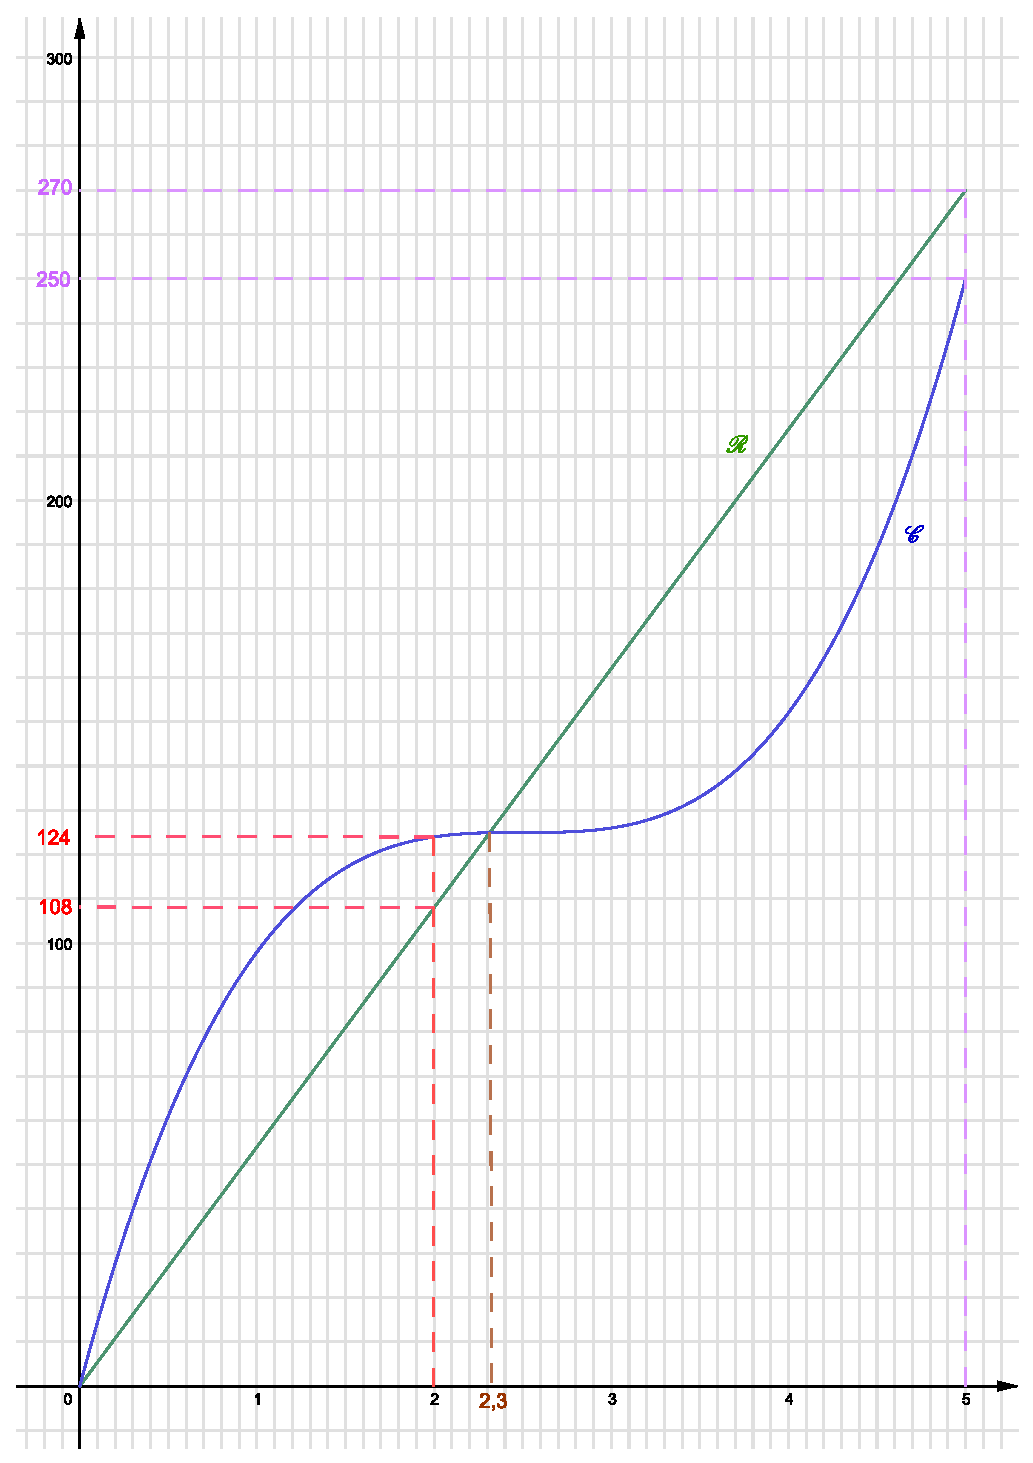
\includegraphics[width=0.9\textwidth]{images/BBESL-s1-2-1c.eps}% gbb 1 unite=3cm
               \end{extern}
          \end{center}
          \cadre{vert}{En pratique}{
               Pour tracer une droite, il suffit de connaître deux points de la droite.
               \par
               Pour obtenir un tracé précis, il est préférable de choisir deux points espacés.
          }
          \par
          \item \`A l'aide du graphique , on voit que~:
          \begin{itemize}
               \item pour une production de 2 tonnes (construction en \textit{rouge})~:
               \begin{itemize}[label=---]
                    \item le coût de fabrication quotidien avoisine \textbf{124~euros} ;
                    \item la recette quotidienne avoisine \textbf{108~euros}.
               \end{itemize}
               \item pour une production de 5 tonnes (construction en \textit{violet})~:
               \begin{itemize}[label=---]
                    \item le coût de fabrication quotidien avoisine \textbf{250~euros} ;
                    \item la recette quotidienne avoisine \textbf{270~euros}.
               \end{itemize}
               \par
          \end{itemize}
          \par
          Dans le premier cas, la recette est inférieure au coût donc l'entreprise est \textbf{déficitaire}.
          \par
          Dans le second cas, la recette est supérieure au coût donc l'entreprise est \textbf{bénéficiaire}.
          \par
          \cadre{rouge}{Bien rédiger}{
               Il n'est pas toujours facile d'expliquer clairement une lecture graphique.
               \par
               Si, comme ici, vous rendez le graphique avec votre copie, \textbf{laissez apparents vos traits de construction} afin que le correcteur puisse comprendre votre démarche.
          }
          \par
          \item L'entreprise réalise un bénéfice lorsque la recette est supérieure au coût de production, c'est à dire lorsque le segment $\mathscr{R}$ est situé au-dessus de la courbe $\mathscr{C}$.
          D'après le graphique, on peut estimer que ceci se produit lorsque $x$ appartient à l'intervalle $[2,3~;~5]$ (tracé en \textit{brun}), c'est à dire pour \textbf{une production supérieure à $\bm{2,3}$ tonnes}.
          \par
     \end{enumerate}
     \par
     %============================================================================================================================
     %
     \TitreC{Partie B}
     %
     %============================================================================================================================
     \par
     \begin{enumerate}
          \item La fonction $C$ est une fonction polynôme sur $[0~;~5]$ donc $C$ est dérivable sur $[0~;~5]$ et~:
          \par
          $C'(x)= 8 \times 3x^2 - 60 \times 2x + 150$\\
          $\phantom{C'(x)}= 24x^2 - 120x + 150.$
          \par
          On peut mettre $6$ en facteur~:
          \par
          $C'(x)= 6(4x^2-20x+25)$.
          \par
          On applique l'identité remarquable $(a-b)^2=a^2-2ab+b^2$~:
          \par
          $C'(x)= 6(2x-5)^2$.
          \par
          Un carré est toujours positif ou nul donc $C'(x) \geqslant 0$ sur $[0~;~5]$.
          \par
          Par conséquent, la fonction $C$ est croissante sur l'intervalle $[0~;~5]$.
          \par
          \cadre{bleu}{Remarque}{
               Il serait tout à fait correct de calculer le discriminant $\Delta$ de la fonction polynôme $C^{\prime}$ pour déterminer son signe.
               \par
               Toutefois, ici, il est préférable et plus rapide de factoriser $C'(x)$ grâce à une identité remarquable.
          }
          \par
          \item
          Le résultat net est la différence entre la recette et le coût de fabrication, donc~:
          \par
          $B(x)=R(x)-C(x)$\\
          $\phantom{B(x)}=54x-(8x^3-60x^2+150x)$\\
          $\phantom{B(x)}=-8x^3+60x^2-96x$
          \par
          $B$ est une fonction polynôme du troisième degré sur $[0~;~5]$ ; elle est donc dérivable et~:
          \par
          $B'(x)=-8\times 3x^2+60\times 2x-96$\\
          $\phantom{B'(x)}=-24x^2+120x-96$.
          \par
          \item \'Etude du signe du trinôme $-24x^2+120x-96$~:
          \par
          $\Delta=120^2-4 \times (-24)\times (-96)=5184=72^2$.
          \par
          Le discriminant est strictement positif donc le trinôme possède deux racines distinctes~:
          \par
          \[ x_1=\dfrac{-120+72}{-2\times (-24)}=1 \quad \text{et} \quad\ x_2=\dfrac{-120-72}{-2\times (-24)}=4. \]
          \par
          Le coefficient de $x^2$ est -24 ; il est négatif, donc $B'(x)$ est négatif à l'extérieur des racines, c'est à dire sur l'ensemble $[0~;~1] \cup [4~;~5]$.
          \par
          De plus~: $B(0)=0 \ ;\ B(1)=-44\ ;\ B(4)=64\ ;\ B(5)=20$.
          \par
          \cadre{vert}{En pratique}{
               Pour obtenir rapidement différentes valeurs de $B(x)$ le plus simple est de saisir la fonction $B$ dans la calculatrice et de faire afficher un tableau de valeurs.
               \par
               Par ailleurs, il est aussi conseillé de tracer le graphique sur la calculatrice pour vérifier le tableau de variations.
          }
          \par
          On en déduit le tableau de signes de $B^{\prime}$ et le tableau de variations de $B$~:
          %:-+-+-+-+- Engendré par~: http://math.et.info.free.fr/TikZ/TableauxVariations/
          \begin{center}
               \begin{extern}%width="450" alt="tableau de variations de la fonction bénéfice"
                    \begin{tikzpicture}[scale=0.875]
                         % Styles
                         \tikzstyle{cadre}=[thin]
                         \tikzstyle{fleche}=[->,>=latex,thin]
                         \tikzstyle{nondefini}=[lightgray]
                         % Dimensions Modifiables
                         \def\Lrg{1.5}
                         \def\HtX{1}
                         \def\HtY{0.5}
                         % Dimensions Calculées
                         \def\lignex{-0.5*\HtX}
                         \def\lignef{-1.5*\HtX}
                         \def\separateur{-0.5*\Lrg}
                         % Largeur du tableau
                         \def\gauche{-1.5*\Lrg}
                         \def\droite{6.5*\Lrg}
                         % Hauteur du tableau
                         \def\haut{0.5*\HtX}
                         \def\bas{-2.5*\HtX-2*\HtY}
                         % Pointillés
                         \draw[dotted,black] (0*\Lrg,\lignex-0.1*\HtX) -- (0*\Lrg,\lignef+0.1*\HtX);
                         \draw[dotted,black] (0*\Lrg,\lignef-0.1*\HtX) -- (0*\Lrg,\bas+0.1*\HtX);
                         \draw[dotted,black] (2*\Lrg,\lignex-0.1*\HtX) -- (2*\Lrg,\lignef+0.1*\HtX);
                         \draw[dotted,black] (2*\Lrg,\lignef-0.1*\HtX) -- (2*\Lrg,\bas+0.1*\HtX);
                         \draw[dotted,black] (4*\Lrg,\lignex-0.1*\HtX) -- (4*\Lrg,\lignef+0.1*\HtX);
                         \draw[dotted,black] (4*\Lrg,\lignef-0.1*\HtX) -- (4*\Lrg,\bas+0.1*\HtX);
                         \draw[dotted,black] (6*\Lrg,\lignex-0.1*\HtX) -- (6*\Lrg,\lignef+0.1*\HtX);
                         \draw[dotted,black] (6*\Lrg,\lignef-0.1*\HtX) -- (6*\Lrg,\bas+0.1*\HtX);
                         % Ligne de l'abscisse~: x
                         \node at (-1*\Lrg,0) {$x$};
                         \node at (0*\Lrg,0) {$0$};
                         \node at (2*\Lrg,0) {$1$};
                         \node at (4*\Lrg,0) {$4$};
                         \node at (6*\Lrg,0) {$5$};
                         % Ligne de la dérivée~: f'(x)
                         \node at (-1*\Lrg,-1*\HtX) {$B'(x)$};
                         \node at (0*\Lrg,-1*\HtX) {$$};
                         \node at (1*\Lrg,-1*\HtX) {$-$};
                         \node at (2*\Lrg,-1*\HtX) {$0$};
                         \node at (3*\Lrg,-1*\HtX) {$+$};
                         \node at (4*\Lrg,-1*\HtX) {$0$};
                         \node at (5*\Lrg,-1*\HtX) {$-$};
                         \node at (6*\Lrg,-1*\HtX) {$$};
                         % Ligne de la fonction~: f(x)
                         \node  at (-1*\Lrg,{-2*\HtX+(-1)*\HtY}) {$B(x)$};
                         \node (f1) at (0*\Lrg,{-2*\HtX+(0)*\HtY}) {$0$};
                         \node (f2) at (2*\Lrg,{-2*\HtX+(-2)*\HtY}) {$-44$};
                         \node (f3) at (4*\Lrg,{-2*\HtX+(0)*\HtY}) {$64$};
                         \node (f4) at (6*\Lrg,{-2*\HtX+(-2)*\HtY}) {$20$};
                         % Flèches
                         \draw[fleche] (f1) -- (f2);
                         \draw[fleche] (f2) -- (f3);
                         \draw[fleche] (f3) -- (f4);
                         % Encadrement
                         \draw[cadre] (\separateur,\haut) -- (\separateur,\bas);
                         \draw[cadre] (\gauche,\haut) rectangle  (\droite,\bas);
                         \draw[cadre] (\gauche,\lignex) -- (\droite,\lignex);
                         \draw[cadre] (\gauche,\lignef) -- (\droite,\lignef);
                    \end{tikzpicture}
               \end{extern}
          \end{center}
          \item Le tableau de variations précédent montre que $B$ atteint un maximum de 64 pour $x=4$.
          \par
          Le résultat net de l'entreprise est donc maximal pour une production de 4 tonnes de granulés.
          \par
          Ce maximum vaut alors 64 centaines d'euros soit $6\ 400$~euros.
          \par
     \end{enumerate}
\end{corrige}

\end{document}